%% LyX 2.3.2 created this file.  For more info, see http://www.lyx.org/.
%% Do not edit unless you really know what you are doing.
\documentclass[12pt,english]{article}
\usepackage[T1]{fontenc}
\usepackage[latin9]{inputenc}
\usepackage{geometry}
\geometry{verbose,tmargin=2cm,bmargin=2cm,lmargin=2cm,rmargin=2cm}
\pagestyle{plain}
\usepackage{array}
\usepackage{wrapfig}
\usepackage{booktabs}
\usepackage{calc}
\usepackage{amsmath}
\usepackage{amssymb}
\usepackage{graphicx}
\usepackage{esint}

\makeatletter

%%%%%%%%%%%%%%%%%%%%%%%%%%%%%% LyX specific LaTeX commands.
%% Because html converters don't know tabularnewline
\providecommand{\tabularnewline}{\\}

\makeatother

\usepackage{babel}
\begin{document}

\section{Introduction}

\textbf{\small{}The goal is to create an operational wildland fire
model that captures fireline behaviors that have been observed in
other models and experiments at a much smaller computational cost. }{\small\par}

Wildfires are multiscale systems with complex dynamics and feedback
mechanisms, making it difficult to capture all of their characteristics.
Physics based models, such as HIGRAD/FIRETEC \cite{linn1997firetec}
(H/F), model the fluid dynamics, the fire-atmosphere interaction,
and the chemical processes (pyrolysis) of fires. These models can
simulate a wide range of conditions but come with large computational
costs and highly complex initialization. This means these models do
not lend themselves to be used for exploring the development of a
fire under slightly varying conditions without a considerable investment
of time. Current operational fire models, used to forecast development
of active fires, are mostly based off the Rothermel spread model,
an empirical model originally developed in 1972. The Rothermel model
has The aim of this research is to develop models that are 

\section{Interface Tracking Model}

We cast the modeling of fire as an interface tracking problem where
a fireline is represented as either a single closed curve (entire
interior burning) ,$\Gamma_{0}$, or as an outer fireline with one
or multiple inner firelines (regions of exhausted or unburnt fuel),
$\Gamma_{i}$ for $i\geq1$. We assume that any burning section of
fuel can be encapsulated with a somewhat smooth continuous curve.
The firelines, $\Gamma_{i},$ represent the isotherm encapsulating
the area where steady combustion of fuel is taking place, $\Omega$. 

We considered three drivers for determing spread rate. The first being
the heat flux of combusting fuel. As fuel combusts it releases radiation
that heats surrounding fuel to ignition temperature, which varies
and ranges from (NEED CITATION AND VALUES). This radiation dries out
surrounding fuel and allows for combustion to take place, allowing
the fire to spread. The heat from wildfires raises the temperature
of the surrounding air causing it to rise(NEED CITATION AND VALUES).
These buoyant updrafts pull in surrounding air at the ground level
that result in a vacuum effect, restraining the spread of the fireline.
The radiation received by fuels is unimpeded by the wind so we considered
these factors separately. Lastly, we account for the background wind
speed that is typically always present in the event of a wildfire.

The fireline model represents the fire dynamics in terms of a normal
velociy, $\frac{\partial\vec{x}}{\partial t}=V_{n}\hat{n},$ where
$\vec{x}$ is a parameterization of a fireline in $\mathbb{R}^{2}$,
and $\hat{n}$ is the outward unit normal of this interface. The normal
velocity$V_{n}$ is represented as the weighted sum from three of
the dominating sources of fire spread:
\begin{align*}
V_{n}(\vec{x}) & =\lambda_{1}v_{bg}(\vec{x})+\lambda_{2}v_{F}(\vec{x})+\lambda_{3}v_{Sink}(\vec{x}).
\end{align*}
\begin{wrapfigure}{R}{0.5\columnwidth}%
\begin{centering}
\fbox{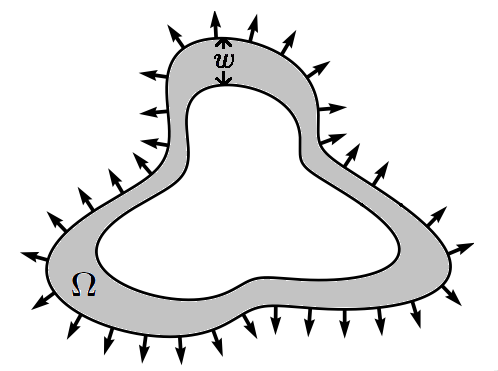
\includegraphics[width=0.45\textwidth]{figures/DomainSchem}}
\par\end{centering}
\small

\caption{Diagram of an expanding fireline interface with a single inner and
outer fireline. The burning region $\Omega$ is shaded in gray, normal
velocity vectors in black, and the width, $w$, defined as the shortest
distance for a point on the exterior to a point on the interior.\label{fig:InterfaceSchem}}

\end{wrapfigure}%

The spread due to the heat flux of burning fuel is denoted by $v_{F}$,
the convective sinks caused by updrafts are represented by $v_{Sink}$,
and the ambient background wind near the ground is represented by
$v_{bg}$.

\subsection{Dynamics}

\subsubsection{Heat Flux}

For the transfer of heat from a source we follow the inverse square
law. To determine the total heat flux at a single point on the interface
we integrate over the enclosed area of the interface. 

\[
v_{F}(\vec{x})=\int_{\Omega}\frac{1}{\sqrt{\left\Vert \vec{x}-\vec{y}\right\Vert ^{2}+\epsilon^{2}}}dA
\]

For this project we originally focused on fires with one interior
fireline. With only one interior fireline the integral can be approximated
by determining the width ,$w_{i}$, of the burning region between
the inner and outer fireline at each discretization point. The width
is defined as the distance between a point on the outer fireline and
the closest point on the inner fireline. The closest point is determined
by doing a few Newtons method iterations in Fourier space\footnote{Should i explain this further?}
to find the $\alpha_{i}$ where $\partial\left(\Gamma_{0}^{i}-\Gamma_{1}\right)/\partial\alpha=0$
that is nearest to $i\frac{2\pi}{N}$ where \textit{N} is the number
of discretization points. With the corresponding alpha the FFT weights
are used to return back to physical space by summing the corresponding
exponentials. With the nearest interior points determined we also
define the midpoints, $y_{i},$ as the halfway point between the outer
point and its associated nearest interior point. These points will
be used as the source locations for calculating the effect of the
convective sinks.

INSERT GRAPHIC OF NEAREST NEIGHBOR RESULTS AND POINTS

The heat flux can now be calculated as a line integral along the outer
fireline using the width to calculate the area of the enclosed burning
region.

\[
v_{F}(\vec{x})=\ointop_{\Gamma_{0}}\frac{w(\vec{y})}{\sqrt{\left\Vert \vec{x}-\vec{y}\right\Vert ^{2}+\epsilon^{2}}}d\vec{s}\,\,\text{for}\,\vec{y}\in\Gamma_{0}.
\]

This integral is calculated by first determing \textit{ds} by taking
the spectral derivative of the outer interface. The guaranteed periodicity
of the interface means we can calculate its derivatives in Fourier
space making the calculation trivial and spectrally accurate\footnote{Explain this in more detail?}.
Given we can express a function as the sum of complex exponentials
using the discrete Fourier transform (DFT)
\[
f(x)\simeq\sum_{k=-N/2+1}^{N/2}\hat{f}_{k}e^{ikx}
\]
where $\hat{f}_{k}$ are the weights given by the DFT. The derivative
can be easily approximated by scaling the weights by \textit{ik} and
taking the inverse Fourier Transform (IFT) since
\[
g(x)=\frac{df}{dx}\simeq\sum_{k=-N/2+1}^{N/2}ik\hat{f}_{k}e^{ikx}\Longrightarrow\hat{g}_{k}=ik\hat{f}_{k}.
\]

Using the spectral derivative we can easily approximate $d\vec{s}=\sqrt{\left(\frac{dx}{d\alpha}\right)^{2}+\left(\frac{dy}{d\alpha}\right)^{2}}\hat{\tau},$
where $\Gamma_{0}=\left(x(\alpha),y(\alpha)\right)$, and sum to approximate
the integral
\[
v_{F}(\vec{x}_{j})=\sum_{i=0}^{N-1}\frac{w(\alpha_{i})*ds_{i}*\left(2\pi/N\right)}{\sqrt{\left\Vert \vec{x}_{j}-\vec{y_{i}}\right\Vert ^{2}+\epsilon^{2}}}.
\]


\subsubsection{Fire-Atmosphere Interactions}

To model the effects of buoyant updrafts we considered a DONT KNOW
WHAT TO CALL IT.

\[
v_{Sink}(\vec{x})=-\sum_{i=1}^{N}w(\vec{y}_{i})\frac{\vec{x}-\vec{y}_{i}}{\left\Vert \vec{x}-\vec{y}_{i}\right\Vert ^{2}}\cdot\hat{n}
\]

\begin{wrapfigure}{O}{0.55\columnwidth}%
\begin{centering}
\fbox{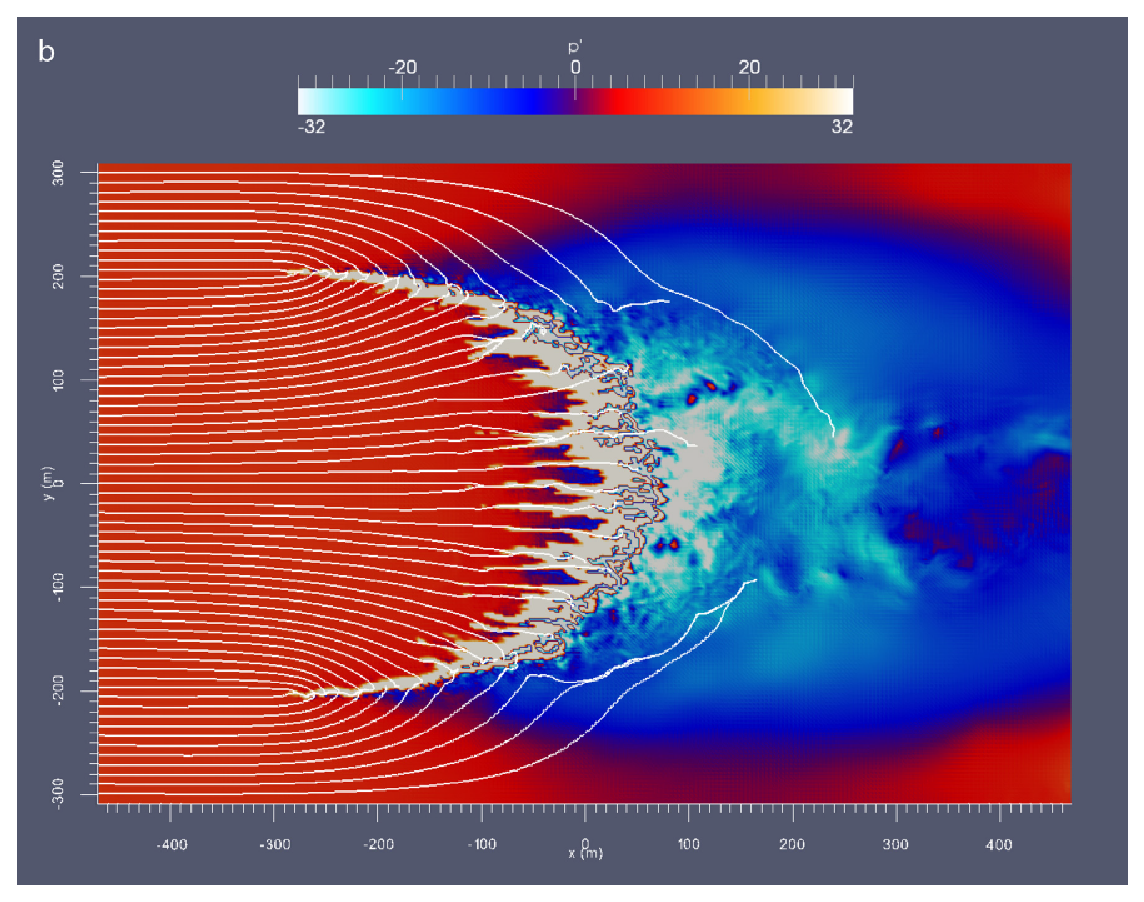
\includegraphics[height=0.1275\paperheight]{figures/CannfieldSinks}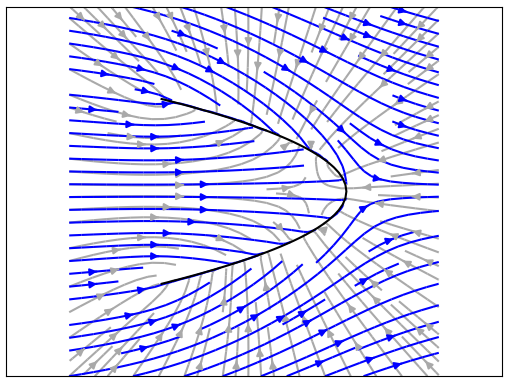
\includegraphics[height=0.13\paperheight]{figures/sinkBoth}}
\par\end{centering}
\small

\caption{A comparison of streamlines from a HIGRAD/FIRETEC \cite{linn1997firetec}
high-fidelity simulation (left) and streamlines from the interface
model (right). The streamlines of the convective sinks are plotted
in gray and the streamlines of $\lambda_{1}\vec{v}_{bg}+\lambda_{3}\vec{v}_{sink}$
$\left(\lambda_{1}=26.6;\lambda_{3}=1.0\right)$ are plotted in blue.
This figure demonstrates that with proper scaling of the convective
sink strength a similar velocity field to a high-fidelity model can
be attained.\label{fig:SinkComparison}}
\end{wrapfigure}%

The larger a burning region the greater the heat released from combustion,
resulting in a stonger convective plume. For a fire with only a single
interior fireline the width is used as a way to scale the convective
sinks. The sum of all of these sinks with their strength, also scaled
by distance, forms the convective sink contribution to the interface
velocity. For firelines with multiple interior lines a Delauney triangulation
was used to mesh the interior burning region. The centers were used
as the sink locations and their strength scaled up by the corresponding
triangles area. The sum over these triangles and the same $r^{-1}$
distance scaling was used to form the convective sink velocity contribution
in these cases.

\subsection{Stability}

A numerical issue with modeling a fireline as a moving interface is
the distortion of the mesh as the interface moves. This leads to a
varying spatial resolution and can cause tangling and instabilities.
By using methods for curvature driven flow\cite{hou1994Ltheta} a
tangential velocity component is introduced that guarantees points
remain equispaced in arclength without affecting the shape of the
interface (Figure ). With this formulation, a well-behaved mesh is
attained and a larger number of stable timesteps can be taken. 

\subsubsection{L-$\theta$ Formulation}

With $\Gamma$ given by $X=\left(x\left(\alpha,t\right),y\left(\alpha,t\right)\right)$
a tangential velocity, $v_{s},$ is introduced to keep the points
along the intereface equispaced in arclength; $X_{t}=v_{n}\hat{n}\rightarrow X_{t}=v_{n}\hat{n}+v_{s}\hat{s}$,
where $\hat{s}$ is the unit tangent vector. To do this a switch of
parameterization of $\Gamma$ from \textit{x} and \textit{y} to the
tangent angle, $\theta,$ and arclength \textit{s}, more specifically
$\frac{\partial s}{\partial\alpha}$. With curvature driven flow $v_{n}=\kappa=\theta_{\alpha}/s_{\alpha}$
we can express the evolution of the curve in terms of $\theta$ and
$s_{\alpha}$via
\begin{equation}
s_{\alpha t}=\left(v_{s}\right)_{\alpha}-\frac{1}{s_{\alpha}}\theta_{\alpha}^{2}\label{eq:sAlphaT}
\end{equation}
\begin{equation}
\theta_{t}=\frac{1}{s_{\alpha}}\left(\frac{1}{s_{\alpha}}\theta_{\alpha}\right)_{\alpha}+\frac{v_{s}}{s_{\alpha}}\theta_{\alpha}.\label{eq:thetaT}
\end{equation}
 We can see that Eq. \ref{eq:thetaT} is an advection-diffusion equation
with stability condition $\Delta t<C\cdot\left(\bar{s_{\alpha}}h\right)^{2}$where
$\bar{s_{\alpha}=\min_{\alpha}s_{\alpha}}$ and \textit{h} is the
grid spacing in $\alpha.$ The stiffness of the problem comes through
Eq. (2) which can be dealt with by ensuring $s_{\alpha}$ doesn't
depend on $\alpha$. To achieve this enforce that $\frac{ds}{d\alpha}$
be everywhere equal to its mean
\[
s_{\alpha}(\alpha,t)=\frac{1}{2\pi}\int_{0}^{2\pi}s_{\alpha'}\left(\alpha^{'},t\right)d\alpha'=\frac{1}{2\pi}L(t)
\]
where $L(t)$ is the total length of the interface $\Gamma$. If $s_{\alpha}$
initially satisfies this constraint then 
\[
v_{s}(\alpha,t)=v_{s}(0,t)+\frac{2\pi}{L}\int_{0}^{\alpha}\theta_{\alpha'}^{2}d\alpha'-\frac{\alpha}{L}\int_{0}^{2\pi}\theta_{\alpha'}^{2}d\alpha',
\]
 resulting from IDONTKNOW, maintains the constraint in time. The tangential
velocity $v_{s}(0,t)$ is an arbitrary change of frame and can simply
be set to zero. Now $s_{\alpha}$ does not depend on $\alpha$ and
evolves with the length of the curve \textit{L}. Eqn. \ref{eq:sAlphaT}
now becomes an ODE for \textit{L} and we now have 
\begin{equation}
L_{t}=-\frac{1}{L}\int_{0}^{2\pi}\theta_{\alpha'}^{2}d\alpha'\label{eq:Lt'}
\end{equation}

\begin{equation}
\theta_{t}=\left(\frac{2\pi}{L}\right)^{2}\theta_{\alpha\alpha}+\frac{2\pi}{L}v_{s}\theta_{\alpha}.\label{eq:thetaT'}
\end{equation}

Substituting the curvature equation and it's derivative with respect
to $\alpha$ into Eqns. \ref{eq:Lt'} and \ref{eq:thetaT'} and using
the restriction $\int_{0}^{2\pi}s_{\alpha'}\left(\alpha^{'},t\right)d\alpha'=L(t)$
we can express our interface evolution in terms of the normal velocity
CITE MOORE
\begin{equation}
L_{t}=-\int_{0}^{2\pi}v_{n}\theta_{\alpha'}d\alpha'\label{eq:FinalLt}
\end{equation}

\begin{equation}
\theta_{t}=\frac{2\pi}{L}\left(v_{n}\right)_{\alpha}+\frac{2\pi}{L}v_{s}\theta_{\alpha}.\label{eq:FinalthetaT}
\end{equation}

\begin{wrapfigure}[18]{O}{0.45\columnwidth}%
\begin{centering}
\fbox{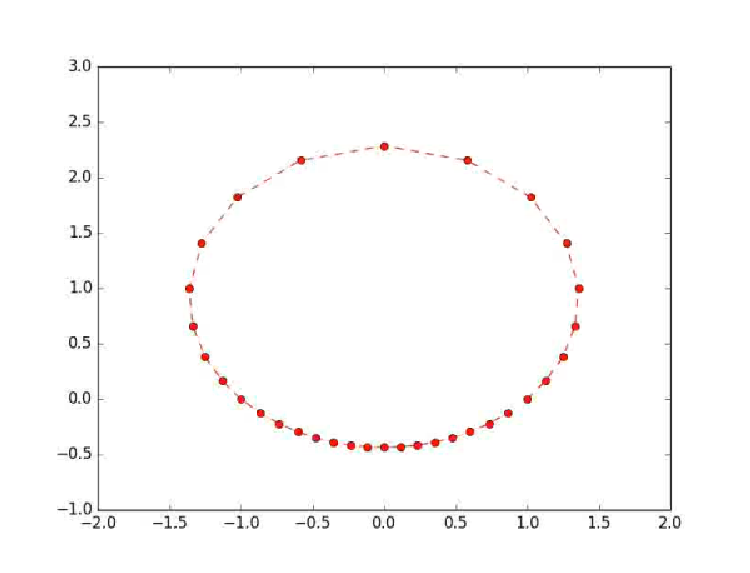
\includegraphics[width=0.2\paperwidth]{figures/noTheta}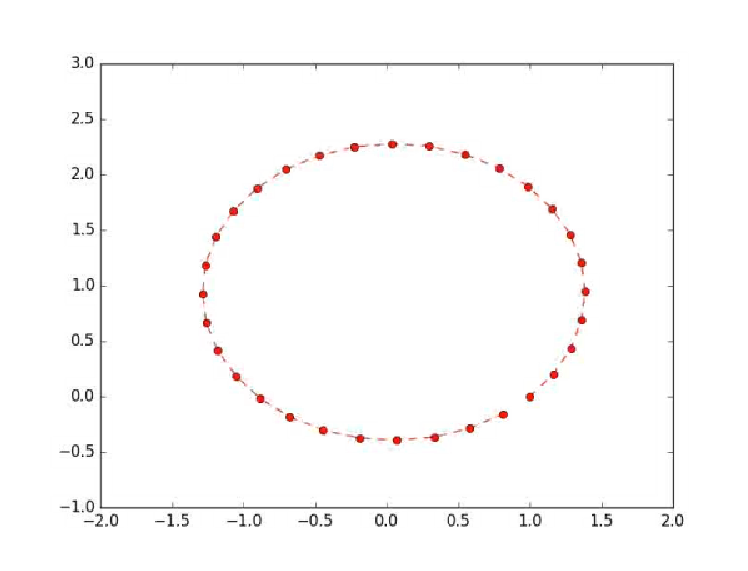
\includegraphics[width=0.2\paperwidth]{figures/Theta}}
\par\end{centering}
\small

\caption{Snapshots of two moving interfaces initialized as a unit circle centered
at the origin with $\vec{v}_{n}(t)=y\hat{n}$. The left interface
has no tangential velocity component and the right interface has the
tangential velocity implemented \cite{hou1994Ltheta}. Notice that
the right interface has the same shape as the left and keeps points
equispaced in arclength.\label{fig:LThetaExample}}
\end{wrapfigure}%

Now $v_{n}$ can be formed using the methods described above section
and with Eqns. \ref{eq:FinalLt} and \ref{eq:FinalthetaT} the discretization
points can be kept equispaced in arclength. Since we are now keeping
track of opening angle and length we need to track a reference point
in cartesian space to account for translations of the interface. For
this we track the surface mean $\left\langle X\right\rangle $ which
moves according to 
\[
\left\langle X\right\rangle _{t}=\left\langle v_{n}\hat{n}+v_{s}\hat{s}\right\rangle 
\]
which is tracked using forward Euler\footnote{Explain this in more detail?}.

Show verification with just translation

Can do error convergence for translation tracking (not necessary)

Could have done optimization of streamline figure to determine lamda1
and lamda2 using firetec results to get time evolution of lambdas(if
they are constant proceed)

\section{Model Fitting with Delayed-Rejection Adaptive-Metropolis}

In an effort to determine a limiting domain for $\lambda$ values
a Delayed-Rejection Adaptive-Metropolis (DRAM) Bayesian inference
algorithm\cite{haario2006dram} was explored. The objective of DRAM
is to start with a prescribed prior distribution and then sample the
parameter space to determine the posterior probability density for
each parameter. This is done by updating the likelihood based on a
prescribed error function defined by the user.

\subsection{Adaptive Metropolis}

In a standard Metropolis algorithm your parameter space is sampled
using a static prior distribution. In Adaptive Metropolis (AM) the
covariance of the proposal distribution is updated after some initial
non-adaptation period, $t_{0}$, based on all of the previous states.
AM is important in the inference procedure since we have no prior
knowledge of what the prior distributions for $\lambda$ are. The
covariance matrix for AM is defined as

\begin{equation}
C_{t}=s_{d}\text{Cov}(X_{0},X_{1},\ldots,X_{t-1})+s_{d}\varepsilon I_{d},
\end{equation}
 where $s_{d}$ is a parameter that depends only on the dimension,
\textit{d},\textit{ }of the the state space where $\pi$ is defined,
$\varepsilon>0$ is a constant, and $I_{d}$ is the \textit{d} dimensional
identity matrix. The constant $\varepsilon$ is there to ensure $C_{t}$
does not become singular, which is small and in practice can typically
be set to zero \cite{haario2001adaptive}. The parameter $s_{d}$
was shown in \cite{sdConf} to optimize the mixing properties of the
Metropolis search in the case of Gaussian targets and Gaussian proposals
when set to $s_{d}=2.4^{2}/d.$ Now if we define $C_{0}$ as a strictly
positive definite initial covariance then we have
\[
C_{t}=\begin{cases}
C_{0} & t\leq t_{0}\\
C_{t}=s_{d}\text{Cov}(X_{0},X_{1},\ldots,X_{t-1})+s_{d}\varepsilon I_{d} & t>t_{0}
\end{cases}.
\]
But at this point it seems quite computationally expensive to calculate
the covariance each step. Luckily if we first look at the definition
of the empirical covariance matrix for $X_{0},\ldots,X_{k}\in\mathbb{R}^{d}$:
\begin{equation}
\text{Cov}(X_{0},\ldots,X_{k})=\frac{1}{k}\left(\sum_{i=0}^{k}X_{i}X_{i}^{T}-(k+1)\bar{X}_{k}\bar{X}_{k}^{T}\right),
\end{equation}
where
\[
\bar{X}_{k}=\frac{1}{k+1}\sum_{i=0}^{k}X_{i}
\]
with \textit{X }being column vectors, we can combine (1) and (2) to
get
\begin{equation}
C_{t+1}=\frac{t-1}{t}C_{t}+\frac{s_{d}}{t}\left(t\bar{X}_{t-1}\bar{X}_{t-1}^{T}-(t+1)\bar{X}_{t}\bar{X}_{t}^{T}+X_{t}X_{t}^{T}+\varepsilon I_{d}\right).
\end{equation}
So it's clear that we can update $C_{t}$ quite easily and the seemingly
computationally expensive term, $\bar{X_{t}},$ follows the simple
recursion relation $\bar{X}_{t}=\frac{t+1}{t}\bar{X}_{t-1}+\frac{1}{t+1}X_{t}.$
This adaptation seems as though it would remove ergodicity, but, was
proven from first principles in \cite{haario2001adaptive} to be ergodic.

With $C_{0}$, $t_{0}$, and $\varepsilon$ have defined at initialization
adaptation in the Metropolis algorithm is achieved. AM provides one
way of improving the naive Metropolis method to handle tougher distributions
to sample that might have issues converging.

\subsection{Delayed Rejection}

With very little prior knowledge on the scale of $\lambda$ parameters
the initial guess for $\lambda$ is most likely a poor one. This may
lead to very slow convergence to a stationary distribution even with
AM implemented. In Delayed Rejection (DR) an alternative move is proposed
upon rejection that is not only dependent on the current state but
also the rejected proposal. In the Metropolis algorithm a candidate
move $Y_{1}$ is generated from a proposal $q_{1}(X|\cdot)$and accepted
with probability
\[
\alpha_{1}(X|Y_{1})=\min\left(1,\frac{\pi(Y_{1})q_{1}(Y_{1}|X)}{\pi(X)q_{1}(X|Y_{1})}\right)=\min\left(1,\frac{N_{1}}{D_{1}}\right).
\]
 When rejected, instead of $X_{t+1}=X$, a second move, $Y_{2}$,
is proposed which is allowed to depend not only on $X$ but $Y_{1}$
as well. The accepted probability is calculated so that reversibility
with $\pi$ is preserved separately at each stage. This allows for
delayed rejection to be interrupted at any stage. The probabilty for
the second stage has the form
\[
\alpha_{2}(X|Y_{1},Y_{2})=\min\left(1,\frac{\pi(Y_{2})q_{1}(Y_{2}|Y_{1})q_{2}(Y_{2}|Y_{1},X)[1-\alpha_{1}(Y_{2}|Y_{1})]}{\pi(X)q_{1}(X|Y_{1})q_{2}(X|Y_{1},Y_{2})[1-\alpha_{1}(X|Y_{1})]}\right)=\min\left(1,\frac{N_{2}}{D_{2}}\right).
\]
We can continue this process and we get an iterative expression of
\[
\alpha_{i}(X|Y_{1},\cdots,Y_{i})=\min\Big(1,\Big\{\frac{\pi(Y_{i})q_{1}(Y_{i}|Y_{i-1})q_{2}(Y_{i}|Y_{i-1},Y_{i-2})\cdots q_{i}(Y_{i}|Y_{i-1},\cdots,X)}{\pi(X)q_{1}(X|Y_{1})q_{2}(X|Y_{1},Y_{2})\cdots q_{i}(X|Y_{1},\cdots,Y_{i})}
\]
\[
\frac{[1-\alpha_{1}(Y_{i}|Y_{i-1})][1-\alpha_{2}(Y_{i}|Y_{i-1},Y_{i-2})]\cdots[1-\alpha_{i-1}(Y_{i}|Y_{i-1},\cdots,Y_{1})]}{[1-\alpha_{1}(X|Y_{1})][1-\alpha_{2}(X|Y_{1},Y_{2})]\cdots[1-\alpha_{i-1}(X|Y_{1},Y_{2},\cdots,Y_{i-1})]}\Big\}\Big)
\]

\[
=\min\left(1,\frac{N_{i}}{D_{i}}\right).
\]
 This is an ugly expression, but a small simplification can be made
to form a recursive formula. If the $i$th stage is reached then we
know $N_{j}<D_{j}$ for $j=1,\cdots,i-1$ therefore $\alpha_{j}(X|Y_{1},\cdots,Y_{j})$
can be rewritten as $\frac{N_{j}}{D_{j}}$ for $j=1,\cdots,i-1$.
This lets us express $D_{i}$ with the recursive formula 
\[
D_{i}=q_{i}(X|Y_{1},Y_{2},\cdots,Y_{i})(D_{i-1}-N_{i-1})
\]
\[
=q_{i}(X|Y_{1},Y_{2},\cdots,Y_{i})[q_{i-1}(X|Y_{1},Y_{2},\cdots,Y_{i-1})[q_{i-2}(X|Y_{1},Y_{2},\cdots,Y_{i-2})\cdots
\]
\[
[q_{2}(X|Y_{1},Y_{2})[q_{1}(X|Y_{1})\pi(X)-N_{1}]-N_{2}]\cdots-N_{i-1}].
\]

\begin{wrapfigure}{R}{0.5\columnwidth}%
\begin{centering}
\fbox{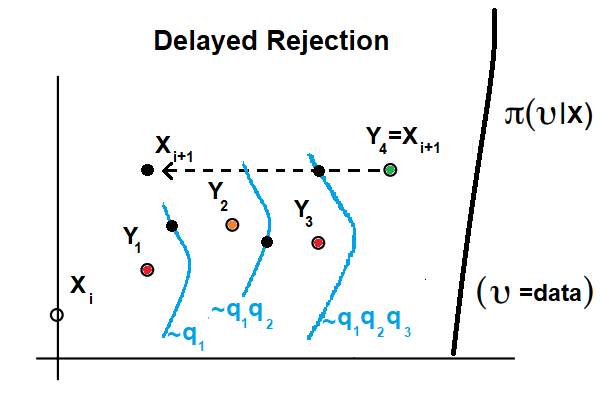
\includegraphics[width=0.4\paperwidth]{figures/DelayedRejection}}
\par\end{centering}
\small

\caption{Diagram of the DR algorithm. Proposals $Y_{1},\,Y_{2},\,\text{and}\,Y_{3}$
were rejected with $Y_{4}$ satisfying the acceptance criteria and
being accepted.\label{fig:DelayedRejectionDiag}}
\end{wrapfigure}%

The amount of times rejection is delayed is up to the user so we can
decide to try at most 4 proposals otherwise let the chain stay where
it is. Above is a diagram of what that process might look like if
thr $4^{th}$ proposal was accepted. An alternative is to have a prescribed
probability \textit{p} of upon rejection moving to a higher stage
proposal. In \cite{tierney1999some} DR was proved to outperform standard
Metropolis-Hastings(MH) in the Peskan absolute efficiency ordering.
This means that DR obtains MCMC estimators that have a smaller asymptotic
variance for every function \textit{f} whose expectation relative
to $\pi$ we want to estimate (provided \textit{f} has finite variance
under $\pi$)\cite{haario2006dram}.

Both DR and AM are standalone modifications made to MCMC methods but
complement eachother well. Putting these two together was shown to
retain ergodicity in \cite{haario2006dram} with some restrictions.
Combining the two (DRAM) is simple, allow the covariance for AM to
be calculated with the DR result.
\begin{center}
\begin{figure}
\begin{centering}
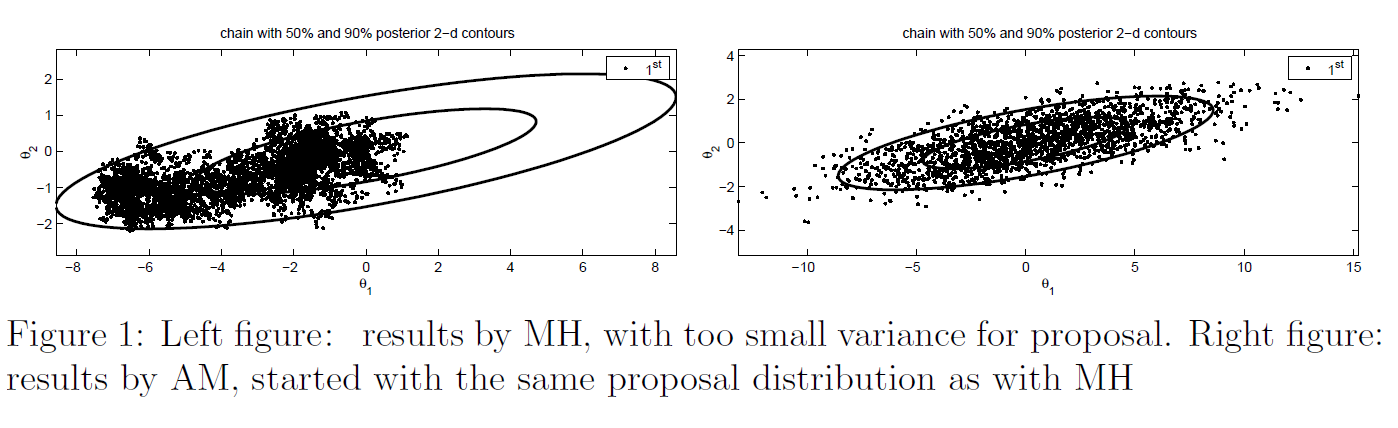
\includegraphics[width=1\textwidth]{figures/HaarioMHAM}
\par\end{centering}
\begin{centering}
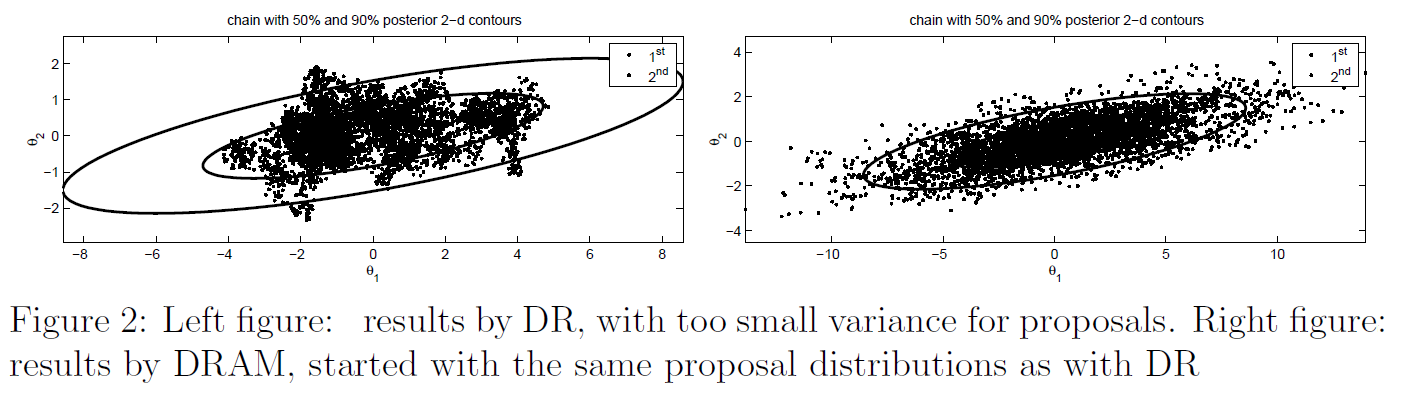
\includegraphics[width=1\textwidth]{figures/HaarioDRDRAM}
\par\end{centering}
\caption{Results from \cite{haario2006dram} that show the how the combination
of DR and AM can outperform MH, DRMH, and AMH on their own. These
figures show DRAMs superior sampling versus when using a proposal
with too small of a variance. \label{fig:HaarioExample}}
\end{figure}
\par\end{center}

It's clear to see that DRAM samples the proposal well in the example
shown in Figure \ref{fig:HaarioExample}, especially against MH and
DRMH. For another demonstration consider noisy data measurements damped
harmonic oscillator. We know the equation of a damped harmonic oscillator
is 
\[
u(t)=e^{-\gamma t}U_{0}\cos(\omega t)
\]
 where $\gamma$ is the damping coefficient, $U_{0}$ is the initial
displacement, and $\omega$ is the angular speed. So we expect the
data to fit this form so we can use Bayesian Inference using true
values, which were used to form the data with some added Gaussian
noise, and the inferred parameters, $\gamma_{i}',U_{0,i}',\omega_{i}'$
at a given step to calculate an error to form the likelihood and make
the next proposal. To test all of these methods I used a code 'MCMC
toolbox' based on \cite{haario2006dram,haario2001adaptive} which
can be found at 'http://helios.fmi.fi/\textasciitilde lainema/mcmc'.
Like the example above I supply reasonable variances to both the $\gamma$
and $U_{0}$ proposals but I assign a very small variance to the $\omega$
proposal distribution. This means that many proposals are rejected
due to $\omega$ not being able to make large enough jumps when a
new set of parameters is sampled.
\begin{center}
\begin{tabular}{|c|c|c|}
\hline 
Parameter & True & Initialized\tabularnewline
\hline 
\hline 
$\gamma$ & 1.2 & 5\tabularnewline
\hline 
$U_{0}$ & 9.7 & 16.7\tabularnewline
\hline 
$\omega$ & 3.4 & 8.2\tabularnewline
\hline 
\end{tabular}
\par\end{center}

Not only is the variance of $\omega$ restricted greatly, but, we'll
start with very poor initial values for the parameters to see if their
is any difference between the methods in locating the distribution
we are after. For each of the methods used 10,000 samples will be
taken and MH was the underlying Metropolis sampling algorithm used
that DR and AM was applied to.
\begin{center}
\begin{tabular}{>{\centering}m{1.5cm}ccc}
\toprule 
Sampling Method & Sampling Paths & Chains & Marginals\tabularnewline
\midrule
\midrule 
MH & 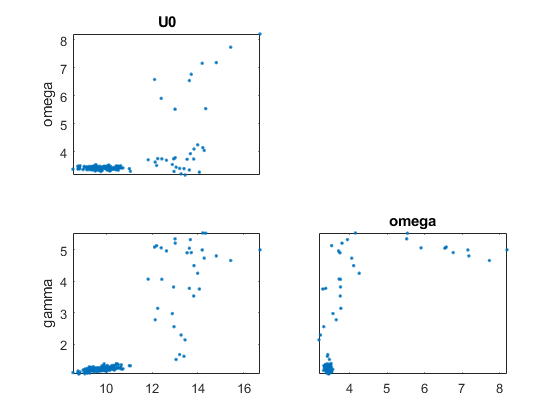
\includegraphics[scale=0.3]{figures/mhMarg} & 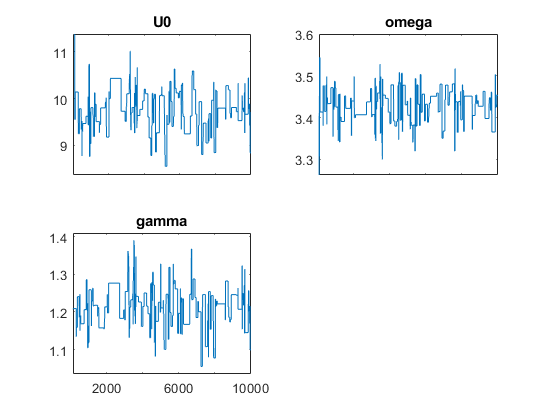
\includegraphics[scale=0.3]{figures/mhChain} & 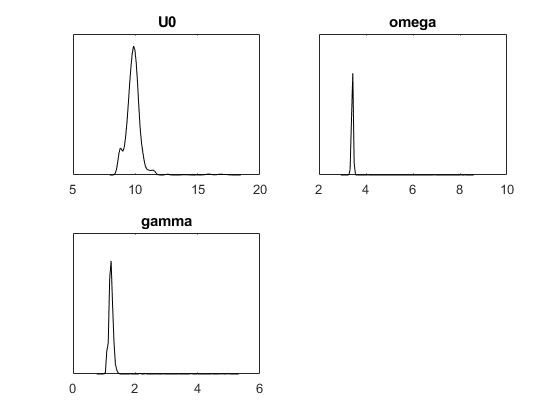
\includegraphics[scale=0.3]{figures/mhDist}\tabularnewline
\midrule
\midrule 
AM & 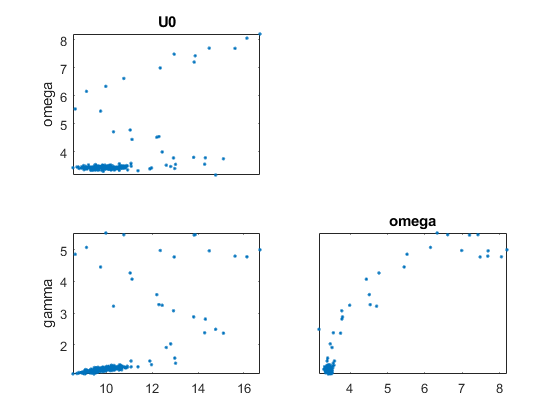
\includegraphics[scale=0.3]{figures/amMarg} & 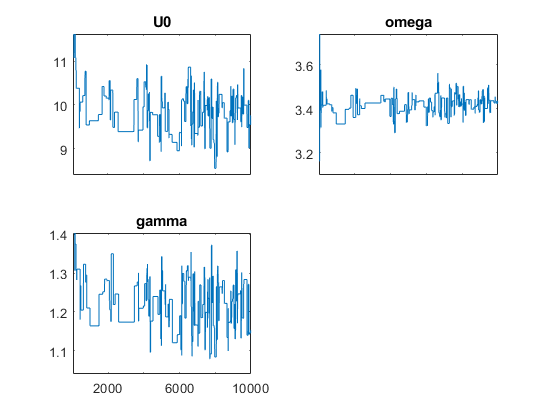
\includegraphics[scale=0.3]{figures/amChain} & 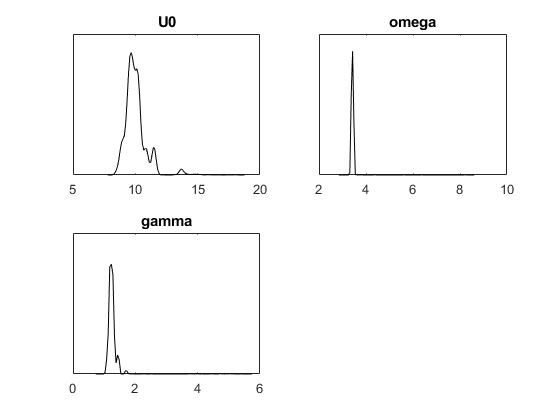
\includegraphics[scale=0.3]{figures/amDist}\tabularnewline
\midrule
\midrule 
DR & 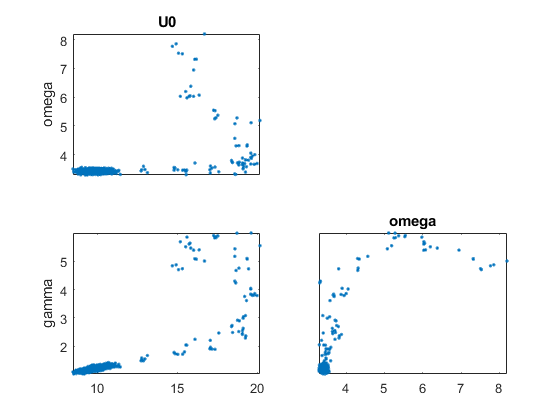
\includegraphics[scale=0.3]{figures/drmarg} & 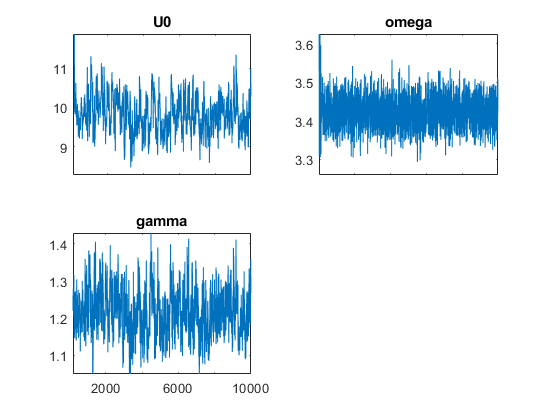
\includegraphics[scale=0.3]{figures/drChain} & 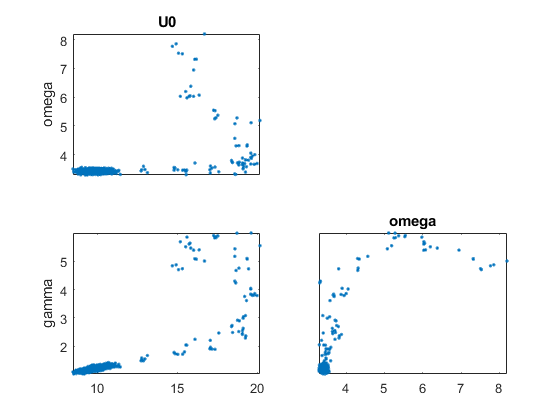
\includegraphics[scale=0.3]{figures/drmarg}\tabularnewline
\midrule
\midrule 
DRAM & 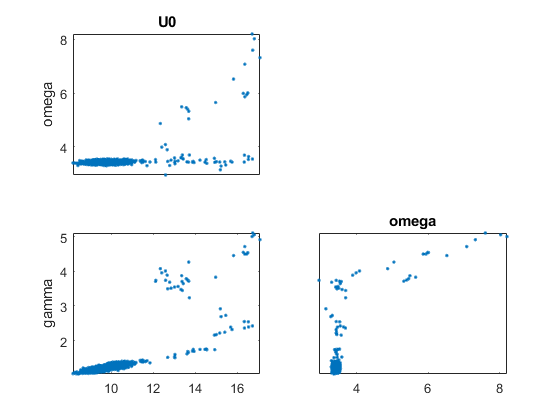
\includegraphics[scale=0.3]{figures/dramMarg} & 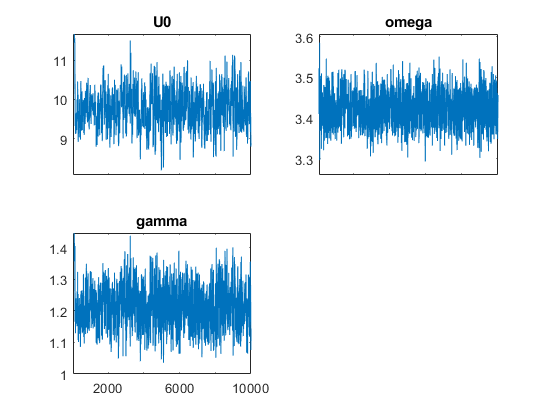
\includegraphics[scale=0.3]{figures/dramChain} & 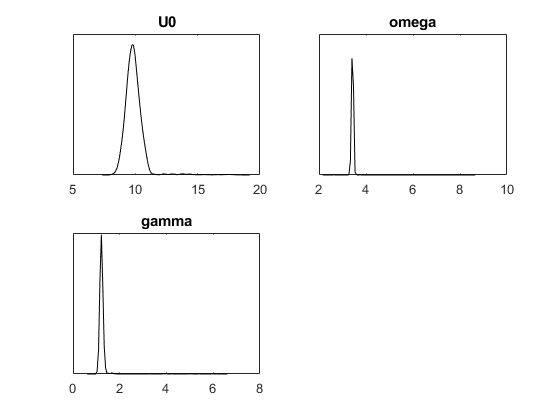
\includegraphics[scale=0.3]{figures/dramDist}\tabularnewline
\bottomrule
\end{tabular}
\par\end{center}

From the plots we can see that both MH and AM have long chains of
rejection. This is not an issue for DR and DRAM and we get good mixing
for these two. From these two examples we can see that when we have
a poor proposal, DR and AM can tune our sampling, but, in the second
example AM's covariance could not adapt to become large enough for
good mixing. Although, near the end of the AM run it seems as though
AM's adaptation began to show its effects and better mixing is seen.

Even though these examples are quite contrived, there is still great
utility in DRAM. Only the variance of $\omega$ was greatly limited
yet strings of rejection were seen in all parameters of MH and AM.
Imagine a high dimensional system that you wanted to perform Bayesian
Inference on. If there is a parameter that you have a poor approximation
for it's variance, then your acceptance of most of the other paramters
will be restricted if everything is coupled. Identifying which parameter
has too limiting of a variance could be like finding a needle in a
haystack. DRAM keeps this from happening, and also with enough time
the adaptation will give you a better approximation for the variance
you should be using in your proposals.

HERE

The DRAM algorithm will show correlations between parameters, shortcomings
of the model, and quantify uncertainty. DRAM requires analysis of
results and reinitialization to attain good stationary posterior distributions.
Depending on the number of inferred parameters, the DRAM algorithm
can require a large amount of simulation runs to estimate these parameters,
and my previous experiences with HPC will prove useful. In addition,
the computational efficiency of this model makes it a natural fit
for DRAM.

The error that was used for driving the model took three points from
a head fire high fidelity simulation from HIGRAD/FIRETEC shown in
\cite{canfield2014numerical} which had the canonical parabolic fireline
shape I was hoping to capture. The initial fireline had a width (x
domain) of 20m and a height (y domain) of 100m, which was similar
to initial conditions in \cite{canfield2014numerical} with a backing
wind of 5 m/s in the positive x-direction. The values used to form
the error function are shown in Table \ref{tab:DRAMpoints}.\begin{wraptable}{o}{0.3\columnwidth}%
\begin{centering}
\begin{tabular}{|c|c|}
\hline 
x & y\tabularnewline
\hline 
\hline 
-30 & 0\tabularnewline
\hline 
544 & 0\tabularnewline
\hline 
{*} & 55\tabularnewline
\hline 
\end{tabular}
\par\end{centering}
\caption{Error points used for error function with the {*} being a free x value.
Once a simulation was completed the min and max x values and max y
values were taken and compared with the three points above. \label{tab:DRAMpoints}}

\end{wraptable}%

Since the initial fire line was initialized with its center being
on the x-axis with a background wind only in the x-direction the developing
fireline would be symmetric with respect to the x-axis as well as
not drift upward. This means that these points were a consistent error
measurement.

There have been many improvements but there seems to be, for lack
of a better term, forbidden regions. There are combinations of $\lambda_{1},$
$\lambda_{2},$ and $\lambda_{3}$ that cause high frequency modes
developing and the interface breaks. This is an obvious obstacle when
using this model with DRAM since if a model returns nonsensical results
how does DRAM update the proposal distribution? Another layer of difficulty
is the fact that this code is written in Python. My solution for this
was to put catch points in my code to detect when the interface had
become unstable. When this happened the simulation was terminated
and a number code was returned instead of a result. In DRAM whenever
this code was received an error of $\infty$ was returned, which the
code is able to handle. My initial fix for this was making modifications
to a significant amount of the DRAM code to have it resample until
it received an actual result. This caused the time to get samples
to increase dramatically. I was able to do 200 runs over a 2 day period
which is a completely inadequate amount of samples to be able to do
any sort of analysis. By making the above change I was able to do
1,000 runs in a 1 day period. All of these runs returned dissappointing
results, although, there is some knowledge gained from using DRAM
with this model.

NEED BETTER RESULTS
\begin{center}
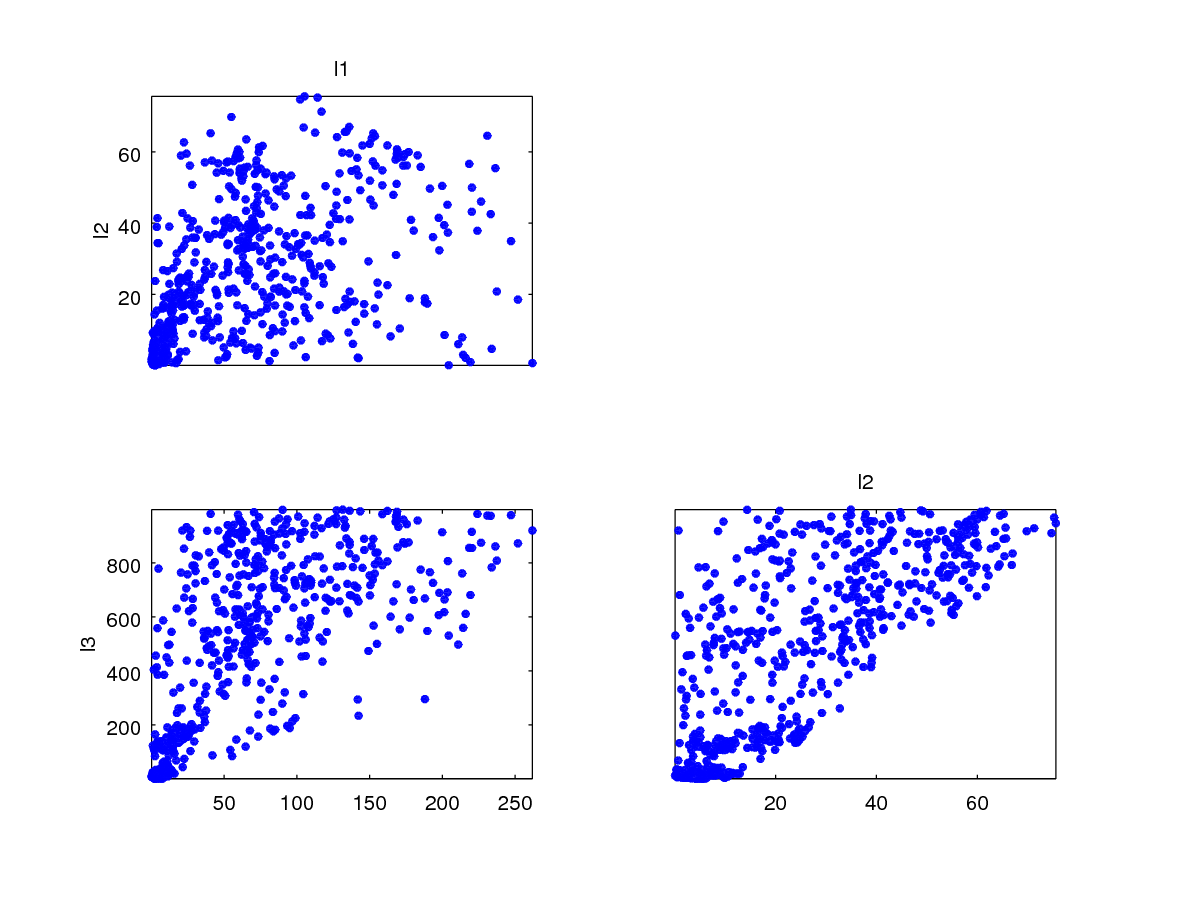
\includegraphics[width=0.6\textwidth]{figures/chains1000}
\par\end{center}

Luckily this is the one that produced some possible information about
the model. From the bottom right plot we can see that there seems
to be an area where DRAM cannot sample. Taking a points from this
graph and fitting a line along the bottom region I arrived at an expression
of 
\[
13.846\lambda_{2}-\lambda_{3}\geq207.6
\]
for the bottom region. Running my simulation with parameters satisfying
this did in fact cause the simulation to break. Taking $\lambda_{1}$
and $\lambda_{2}$ factors from the upperleft plot and taking the
satisfying the negative of the above expression resulted in simulations
that ran the full time and didn't break. Sadly the simulation runs
resulting from the sampling means are not realistic. The final shape
of the resulting fireline does in fact have its width around the right
scale of the data points but it's height is much too large, \textasciitilde 200m.
At least a rough constraint for stability for the model was able to
be realized. This exercise definitely has shown that much more foresight
needs to be used in order to utilize an MCMC sampling algorithm efficiently.

\bibliographystyle{plain}
\bibliography{/home/djr16/References}


\section{SARndbox}

\section{Conclusion}
\end{document}
